\section{Theoretische Grundlage}
\label{sec:Theorie}
Zur Beugung von Licht kommt es, wenn die Abmessung des Hindernisses in der Größenordung der Wellenlänge $\lambda$ des Lichts liegt. Dabei kommt es zur Abweichung des Lichtes von der Geometrischen Optik. Bei der Fresnel-Näherung ist die Lichtquelle und der Beobachtungspunkt nah zusammen, wodurch die Lichtstrahlen nicht um den gleichen Winkel gebrochen werden. Für den Versuch wird angenommen, dass der Schirm sehr weit von der Blende entfernt ist, so dass die Fraunhofer-Näherung genutzt werden kann. In Abbildung \ref{fig:Fra} ist zu sehen, dass das Licht jeweils um den Winkel $\phi$ gebeugt wird.
\begin{figure}
  \centering
  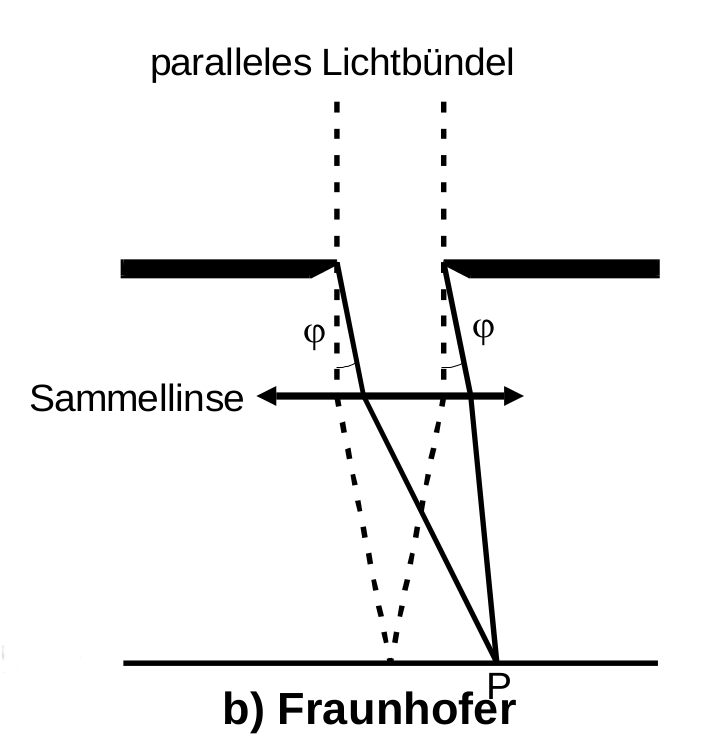
\includegraphics[height=6cm]{picture/Frauenhofer.png}
  \caption{Fraunhofer Beugung. \cite[1]{sample}}
  \label{fig:Fra}
\end{figure}
Anhand des Huygensschen Prinzip lässt sich bei hinreichend großer Intensität die Interferenz beschreiben. Es besagt einerseits, dass jeder Punkt einer Wellenfront Ausgangspunkt einer neuen Kugelwelle ist und andererseits, dass die Einhüllende der Elementarwellen die neue Wellenfront ergibt. Um eine Aussage in einem Punkt zu machen, müssen nach dem Huygensschen Prinzip alle Wellen die in diesem Punkt ankommen überlagert werden. Der einfachheit halber wird zunächst ein Einzelspalt betrachtet und anschließend auf andere Spalte geschlossen. Interferenz bedeutet beim Einzelspalt, dass die einzelnen Amplituden der Elementarwellen, die gleichzeitig in einem Punkt sind, überlagert werden.
\begin{figure}
  \centering
  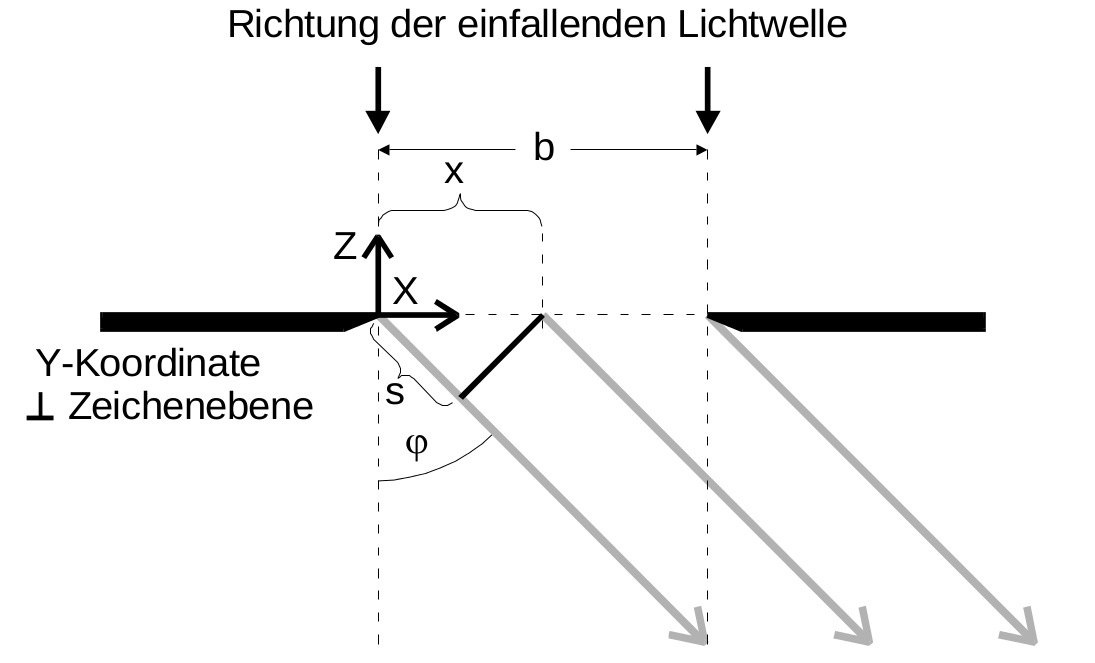
\includegraphics[height=5cm]{picture/doppelspalt.png}
  \caption{Phasenbeziehung zwischen zwei Teilstrahlen \cite[3]{sample}}
  \label{fig:dop}
\end{figure}
Es wird eine ebene Welle mit der Feldstärke
\begin{equation}
  A(z,t)= A_0 \textbf{exp} \left(i \left( \omega t - \frac{2 \pi z}{\lambda}   \right) \right)
  \label{eqn:welle}
\end{equation}
angenommen die durch den Spalt mit Breite $b$ einfällt. Der Phasenunteschied zweier Strahlen, mit dem Abstand $x$ beträgt:
\begin{equation}
  \delta = \frac{2 \pi x sin(\phi)}{\lambda}
  \label{eqn:phase}
\end{equation}
Durch Integration über alle Strahlen die um den Winkel $\phi$ abgelenkt sind ergibt sich:
\begin{equation}
  B(z,t,\phi) = A_0 \textbf{exp} \left( i \left( \omega t - \frac{2 \pi z}{\lambda} \right) \right) \cdot \textbf{exp} \left( \frac{\pi b sin(\phi)}{\lambda} \right)
  \label{}
\end{equation}
Für die experimentelle Auswertung müssen die Exponentialfunktionen nicht weiter betrachtet werden, da diese ausschließlich Informationen über die Phase der Funktion enthalten. Da aufgrund der hohen Lichtfrequenz eine Messung der Amplitude nicht möglich ist muss die Intensitätsverteilung ermittelt werden.
\begin{equation}
  I(\phi) \propto B(\phi)^2 = A_0^2 b^2 \left( \frac{\lambda}{\pi b sin \phi} \right)^2 sin^2 \left( \frac{\pi b sin \phi}{\lambda} \right)
  \label{eqn:I}
\end{equation}
Die Intensitätsverteilung $I(\phi)$ des Doppelspalts beruht darauf, das im Abstand $s$ ein zweiter Einzelspalt der Breite $b$ überlagert wird.
\begin{equation}
  I(\phi) \propto B(\phi)^2 = 4cos^2\left( \frac{\pi s sin(\phi)}{\lambda} \right) \left( \frac{\lambda}{\pi b sin \phi} \right)^2 sin^2 \left( \frac{\pi b sin \phi}{\lambda} \right)
  \label{eqn:Id}
\end{equation}

\subsection{Fehlerrechnung}
Sämtliche Fehler und Fits werden im folgenden mit der Funktion "Lmfit" aus Python berechnet.
